\documentclass[a4paper]{book}
\usepackage{commeunjeustyle}
\begin{document}

\chapter*{Réduction des endomorphismes/matrices carrés}
La réduction d'endomorphisme a pour objectif d'exprimer des matrices et des endomorphismes sous une forme plus simple, par exemple pour faciliter les calculs. 
Réduire un endomorphisme $u\in\LE$, cela correspond à trouver une base de l'espace dans laquelle l'endomorphisme s'exprime simplement. C'est à dire c'est décomposer l'espace $E$ comme somme directe de sous-espaces stables par $u$,
$E = \oplus     _{i=1}^n E_i$ où les $E_i$ sont stables par $u$. On peut donc définir  les endomorphismes $u_{|E_i}$ induits par $u$ sur $E_i$, soit :
 $$\Fonction{u_{|E_i}}{E_i }{E_i}{x}{u(x)}.$$
Comme tout vecteur $\vec{x}\in E$ se décompose de façon unique sous la forme
$\vec{x} =  \vec{x_1} + \dots + \vec{x_n}$, on a:
$$ u(\vec{x}) =  u_{|E_1}(\vec{x_1}) + \dots + u_{|E_n}(\vec{x_n}).$$
Ainsi, l'étude de $u$ se ramène à l'étude des endomorphismes $u_{|E_i}$. L'idée directrice est que les $u_i$ sont plus \defi{simples} que $u$ car définis sur des sous-espaces vectoriels de $E$.\\
En dimension finie, avec une base adaptée à la décomposition en somme directe, soit $\mathcal{B}_1$ base de $E_1$,..., $\mathcal{B}_n$ base de $E_n$, la matrice de $u$ dans la base $\mathcal{B}=(\mathcal{B}_1,\dots,\mathcal{B}_n)$ est :  
$$ [u]_\mathcal{B} =\begin{pmatrix}[u_{|E_1}]_{\mathcal{B}_1}&\mathrm {0}&\cdots &\mathrm {0}\\\mathrm {0}&\mathrm [u_{|E_2}]_{\mathcal{B}_2}&\cdots &\mathrm {0}\\\vdots &\vdots &\ddots &\vdots \\\mathrm {0}&\mathrm {0}&\cdots &[u_{|E_n}]_{\mathcal{B}_n}\end{pmatrix}$$
où $\mathrm {0}$ est la matrice nulle.\\
Dans le cas favorable, les $u_i$ sont des homothéties, c'est à dire $u_{|E_i} =\lambda    _i \mathrm{Id}_{E_i}$. 
$$u(\vec{x})=\lambda_1\vec{x_1}+\dots+\lambda_n\vec{x_n}$$
Dans ce cas, la matrice de $u$ dans la base $\mathcal{B}$ est

$$ [u]_\mathcal{B} = \begin{pmatrix}\lambda_1 \mathrm {I}_{\dim(E_1)}&\mathrm {0}&\cdots &\mathrm {0}\\\mathrm {0}&\lambda_2 \mathrm {I}_{\dim(E_2)}&\cdots &\mathrm {0}\\\vdots &\vdots &\ddots &\vdots \\\mathrm {0}&\mathrm {0}&\cdots &\lambda_n \mathrm {I}_{\dim(E_n)}\end{pmatrix}$$
avec $\lambda_i \mathrm {I}_{\dim(E_i)}= \begin{pmatrix}\lambda_i&0&\ldots &0\\0&\lambda_i&\ddots &\vdots \\\vdots &\ddots &\ddots &0\\0&\ldots &0&\lambda_i\end{pmatrix}$. $ [u]_\mathcal{B} $ est donc une matrice diagonale. On dit que l'endomorphisme $u$ est \impo{diagonalisable}. Dans le cadre du programme, l'essentiel du cours de réduction se limite à l'aspect de diagonalisation. Les méthodes de réduction sont de deux types, qu'il convient de souligner : les premières, de nature géométrique, reposent sur les notions de sous-espace stable et d'éléments propres ; les secondes, de nature algébrique, font appel aux polynômes annulateurs.\\


Par exemple, soit E un $\K $-espace vectoriel et $E_1$, $E_2$ deux sous-espaces vectoriels supplémentaires dans E  ($E = E_1 \oplus E_2$).\\
Le projecteur p (ou la projection) sur $E_1$ parallèlement à $E_2$ est défini par:
$$\Fonction{p}{ E = E_1 \oplus E_2 }{ E}{\vec{x} = \vec{x_1} + \vec{x_2}}{\vec{x_1}}$$
\textit{Nature géométrique} : pour tout $x\in E_1:\quad p(\vec{x})= 1.\vec{x}$ donc  $p_{|E_1}=1 \mathrm{Id}_{E_1}$ et  pour tout $x\in E_2:\quad p(\vec{x})= 0.\vec{x}$ donc  $p_{|E_2}=0 \mathrm{Id}_{E_2}$. La matrice de $p$ dans une base adaptée à $E_1 \oplus E_2$ s'écrit :
$$[p]_\mathcal{B} =\begin{pmatrix}1.\mathrm{I}_r&0\\ 0 &0.\mathrm{I}_{n-r}\end{pmatrix}.$$
\textit{Nature algébrique} : On a $p^2=p$, d'où $p^2-p=0$ et enfin $(p-1.\mathrm{Id}_E)(p-0.\mathrm{Id}_E)=0$. Le polynôme $Q=(X-1).(X-0)$ est un polynôme annulateur de l'endomorphisme $p$ car $Q(p)=0$. Comme $Q$ est scindé simple, on démontrera que de nouveau $p$ est diagonalisable dans une base $\mathcal{B} $ adaptée à $E_1 \oplus E_2$.  


\textit{Notations}
\begin{itemize}
\item $\K $ désigne un corps (ici $\R$ ou $\C$);
\item $E$ désigne un $\K $-espace vectoriel de dimension finie;
\item $\LE$ désigne l'ensemble des endomorphismes de $E$,
  c'est à dire  l'ensemble des applications linéaires de $E$ dans $E$.
\end{itemize}
%\Para{Remarque}
%Au cours précédent, on a vu l'aspect dual entre application linéaire et matrice. A partir d'une application linéaire $u$, on se donne 
%et de l'endomorphisme de Kn défini par X?AX. En particulier, X est un vecteur propre de A pour la valeur propre \lambda     si et seulement si AX=\lambda    X.



\section{Stabilité}
\subsection{D'un sous espace vectoriel : $u(F)\subset F$}

\begin{Definition}[Stable] Soit $u\in \LE$. On dit qu'un sous-espace $F$ de $E$ est \defi{stable} par $u$ si $u(F)\subset F$, c'est à dire :
$$\forall \vec{x}\in F,\quad u(\vec{x})\in F.$$ 
On peut alors définir un endomorphisme $u_{|F}\in \mathcal{L}(F)$ en posant $u_{|F}(\vec{x})=u(\vec{x})$ pour tout $x\in F$. $u_{|F}$ s'appelle l'\defi{endomorphisme induit} par $u$ sur $F$.
\end{Definition}
\begin{Exemple}[Dérivée]
Soit $\phi:f\mapsto f'.$ L'espace vectoriel des fonctions $C^{\infty}$ est stable par $\phi$. 
\end{Exemple}
\begin{Proposition} Soit $F$ un sous-espace vectoriel de $E$ de dimension finie et soit $\mathcal{B}$ une base de $E$ dont les premiers vecteurs, $\mathcal{B}'$,  forment une base de $F$. Alors la matrice de $u$ dans cette base a la forme
$$[u]_{\mathcal{B}}= \begin{pmatrix}
A & B \\ 0 & C
\end{pmatrix}$$
si et seulement si $F$ est stable par $u$. Dans ce cas $A=[u_{|F}]_{\mathcal{B}'}$.
\end{Proposition}
\begin{Proposition}[Diagonalisation par blocs] Soit $E_1\oplus     E_2=E$ de dimension finie avec $E_1$ et $E_2$ stables par $u$. Alors la matrice de $u$ dans une base adaptée $\mathcal{B}=(\mathcal{B}_1,\mathcal{B}_2)$ à la décomposition $E_1\oplus     E_2=E$  a la forme diagonale par blocs
$$[u]_{\mathcal{B}}= \begin{pmatrix}
A & 0 \\ 0 & B
\end{pmatrix}$$
 $A=[u_{|E_1}]_{\mathcal{B}_1}$ et $B=[u_{|E_2}]_{\mathcal{B}_2}$.
\end{Proposition}

\begin{Definition}[Stable] Soit $M\in \MnK$. On dit qu'un sous-espace $F$ de $\M{n}{1}{\K}$ est stable par $M$ si
$$\forall X\in \M{n}{1}{\K},\quad MX \in F.$$
Dans ce cas, $M$ est semblable à une matrice de la forme$\begin{pmatrix}
A & B \\ 0 & C\end{pmatrix}$ avec une matrice de passage de la base canonique à une base adaptée à $F$. 
\end{Definition}
\begin{Proposition}[Diagonalisation par blocs] Soit $E_1\oplus     E_2=\MnK$ avec $E_1$ et $E_2$ stables par $M$. Alors la matrice de $M$ est semblable à la matrice diagonale par blocs, c'est à dire que 
$$M=P \begin{pmatrix}
A & 0 \\ 0 & B
\end{pmatrix}P^{-1}$$ avec $P$ la matrice de passage de la base canonique à une base adaptée $\mathcal{B}=(\mathcal{B}_1,\mathcal{B}_2)$.
\end{Proposition}
\begin{Exemple}[Matrice orthogonal]
$$A=\frac{1}{3}\begin{pmatrix}2 & -1 & 2 \\ 2 &2&-1\\ -1&2&2\end{pmatrix}.$$ Soit $E_1=\mathrm{Vect}<\begin{pmatrix}1\\-1 \\0 \end{pmatrix},\begin{pmatrix}1\\0 \\-1 \end{pmatrix}>$ et $E_2=\mathrm{Vect}<\begin{pmatrix}1\\1 \\1 \end{pmatrix}>$.\\
Pour la stabilité, on vérifie que $$A\begin{pmatrix}1\\-1 \\0 \end{pmatrix}=\begin{pmatrix}1\\0 \\-1 \end{pmatrix}\in E_1$$ et $$A\begin{pmatrix}1\\0 \\-1 \end{pmatrix}=\begin{pmatrix}0\\1 \\-1 \end{pmatrix}=-1\begin{pmatrix}1\\-1 \\0 \end{pmatrix} + 1\begin{pmatrix}1\\0 \\-1 \end{pmatrix}\in E_1.$$
De plus, on a $A\begin{pmatrix}1\\1 \\1 \end{pmatrix}=\begin{pmatrix}1\\1 \\1 \end{pmatrix}\in E_2.$\\
$A$ est semblable à la matrice $\begin{pmatrix}0 & -1 & 0 \\ 1 &1&0\\0&0&1\end{pmatrix}$ et la matrice de passage est $P=\begin{pmatrix}1 &1 & 1 \\ -1 &0&1\\0&-1&1\end{pmatrix}$.
\end{Exemple}
\subsection{D'une droite vectoriel : $u(\K \vec{x})\subset \K \vec{x}$ (vecteurs propres et valeurs propres: $u(\vec{x})=\lambda \vec{x}$)}
\begin{Proposition}[Caractérisation] Soit $u\in \LE$. Soit $\vec{x}\in E$.\\
$\K \vec{x}$ est stable par $u$ si et seulement si il existe $\lambda$ dans $\K $ tel que $u(\vec{x})=\lambda \vec{x}$.
\end{Proposition}
\begin{Proposition}[Caractérisation] Soit $M\in \MnK$. Soit $X\in\M{n}{1}{\K}$.\\
 $\K X$ est stable par $M$ si et seulement si il existe $\lambda$ dans $\K $ tel que $MX=\lambda X$.
\end{Proposition}
\begin{Definition}
Soit $u\in \LE$.
\begin{itemize}
\item On dit que $\lambda    \in \K $ est une \defi{valeur propre} de $u$ si  il existe $\vec{x}\neq \vec{0}_{E}$ tel que $u(\vec{x}) =\lambda    \vec{x}$.
\item On dit que $\vec{x}\in E$ est un \defi{vecteur propre} de $u$ associé à la valeur propre $\lambda    $ si  $\vec{x}\neq \vec{0}_{E}$ et $u(\vec{x}) =\lambda    \vec{x}$.
\item On appelle \defi{spectre} de $u$, noté $\mathrm{Sp}(u)$, l'ensemble des valeurs propres de $u$.
\item On appelle \defi{sous-espace propre} de $u$ associé à la valeur propre $\lambda    $ le sous-espace vectoriel $E_\lambda    (u) = \Ker(u -\lambda    \mathrm{Id}_E)$.
\end{itemize}
\end{Definition}

\begin{Exemple} Soit $\Fonction{\Psi}{\mathbb {R}_n[X] }{\mathbb {R}_n[X]}{P}{XP'}$. On a $\Psi(X^i)=i\times  X^i$, pour tout $i\in\{0,\dots,n\}$. $X^i$ est un vecteur propre associé à la valeur propre $i$.
\end{Exemple}
\begin{Exemple} Soit $\phi:f\mapsto f'.$ On a $\mathrm{Sp}(\phi)=\R$. En effet, pour tout $\lambda\in\R$, la fonction $x\mapsto e^{\lambda x}$ est vecteur propre $$\phi(e^{\lambda x})=(e^{\lambda x})'=\lambda e^{\lambda x}.$$
\end{Exemple}
\begin{Definition}
Soit $M\in \MnK$.
\begin{itemize}
\item On dit que $\lambda    \in \K $ est une \defi{valeur propre} de $M$ si  il existe $X\neq \{0_{\M{n}{1}{\K}}\}$ tel que $MX =\lambda    X$.
\item On dit que $X\in\M{n}{1}{\K}$ est un \defi{vecteur propre} de $u$ associé à la valeur propre $\lambda    $ si et seulement si $X\neq 0_{\M{n}{1}{\K}}$ et $MX =\lambda    X$.
\item On appelle \defi{spectre} de $M$, noté $\mathrm{Sp}(M)$, l'ensemble des valeurs propres de $M$.
\item On appelle \defi{sous-espace propre} de $M$ associé à la valeur propre $\lambda    $ le sous-espace vectoriel $E_\lambda    (M) = \Ker(M -\lambda    \mathrm{I}_n)$.
\end{itemize}
\end{Definition}
\begin{Exemple} La matrice $M=\begin{pmatrix}0&1\\1&0\end{pmatrix}$ représente la symétrie par rapport à la première bissectrice, soit la symétrie par rapport à $E_1=\mathrm{Vect}\begin{pmatrix}
1\\1
\end{pmatrix}$ parallèlement à $E_2=\mathrm{Vect}\begin{pmatrix}1\\-1
\end{pmatrix}$.\\
%\begin{center}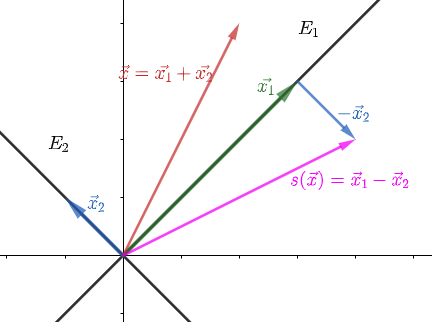
\includegraphics[width=6cm]{symetrie.png}
%\end{center}
On a $M\begin{pmatrix}1\\1\end{pmatrix}=1\begin{pmatrix}1\\1\end{pmatrix}$  et $M\begin{pmatrix}1\\-1\end{pmatrix}=-1\begin{pmatrix}1\\-1\end{pmatrix}$.
$\begin{pmatrix}1\\1\end{pmatrix}$ est un vecteur propre associé à la valeur propre $1$ (tout vecteur appartenant à la première bissectrice est invariant par $M$) et $\begin{pmatrix}-1\\1\end{pmatrix}$ est un vecteur propre associé à la valeur propre $-1$ (tout vecteur orthogonal à la première bissectrice est transformé en son opposé par $M$).
\end{Exemple}
\begin{Proposition}
Soit $u\in \LE$ et $\lambda    \in \mathrm{Sp} u$.\\
Alors l'ensemble des vecteurs propres de $u$ associés à la valeur propre $\lambda    $ est $\Ker(u-\lambda    \mathrm{Id}_E)\setminus\{ \vec{0}_{E}\} $.
\end{Proposition}
\begin{Proposition}
Soit $M\in \MnK$ et $\lambda    \in \mathrm{Sp} M$.\\
Alors l'ensemble des vecteurs propres de $M$ associés à la valeur propre $\lambda    $ est $\Ker(M-\lambda    \mathrm{I}_n) \setminus \{0_{\M{n}{1}{\K}}\}$.
\end{Proposition}

\begin{Proposition}
Soit $u\in \LE$. Les conditions suivantes sont équivalentes:
\begin{itemize}
\item $\lambda    \in \mathrm{Sp} u$;
\item $\exists \vec{x}\neq  \vec{0}_{E}$ tel que $(u -\lambda    \mathrm{Id}_E)(\vec{x}) = \vec{0}_E$;
\item $E_\lambda    (u) = \Ker(u -\lambda    \mathrm{Id}_E)\neq \{ \vec{0}_{E}\}$;
\item $u -\lambda    \mathrm{Id}_E$ n'est pas injective
\item $u -\lambda    \mathrm{Id}_E$ n'est pas bijective (uniquement en dimension finie).
\end{itemize}
\end{Proposition}
\begin{Proposition}
Soit $M\in \MnK$. Les conditions suivantes sont équivalentes:
\begin{itemize}
\item $\lambda    \in \mathrm{Sp} M$;
\item $\exists X\neq 0_{\M{n}{1}{\K}}$ tel que $(M -\lambda    \mathrm{I}_n)X = 0$;
\item $E_\lambda    (M) = \Ker(M -\lambda    \mathrm{I}_n)\neq\{0\}$;
\item $(M -\lambda    \mathrm{I}_n)$ n'est pas inversible.
\end{itemize}
\end{Proposition}

\begin{Proposition}
Soit $u\in \LE$, $\lambda    $ une valeur propre de $u$ et $E_\lambda    $ le sous-espace propre correspondant.\\
Alors $E_\lambda    $ est stable par $u$.\\
De plus, l'endomorphisme induit par $u$ sur $E_\lambda    $ est l'homothétie de rapport $\lambda    $.
Autrement dit, $u_{\vert E_\lambda    } =\lambda    \mathrm{Id}_{E_\lambda    }$.\\
De plus, en dimension finie, la matrice de $u$ dans une base adaptée à $E_\lambda    $ est de la forme :
$$\begin{pmatrix}
\mathrm{I}_{\dim(E_\lambda)} & B \\ 0 & C
\end{pmatrix}.$$ 
\end{Proposition}
\begin{Proposition}[Diagonalisation] Soit $E_{\lambda_1}\oplus E_{\lambda_2}\dots \oplus E_{\lambda_p}  =E$ de dimension finie avec $E_{\lambda_1}$, $E_{\lambda_2}\dots$ et $E_{\lambda_p}$  des espaces propres de $u$. Alors la matrice de $u$ dans une base adaptée à $E_{\lambda_1}\oplus E_{\lambda_2}\dots \oplus E_{\lambda_p}$ est :
$$ \begin{pmatrix}\lambda_1 \mathrm {I}_{\dim(E_1)}&\mathrm {0}&\cdots &\mathrm {0}\\\mathrm {0}&\lambda_2 \mathrm {I}_{\dim(E_2)}&\cdots &\mathrm {0}\\\vdots &\vdots &\ddots &\vdots \\\mathrm {0}&\mathrm {0}&\cdots &\lambda_p \mathrm {I}_{\dim(E_p)}\end{pmatrix}.$$
\end{Proposition}

\begin{Proposition}
Soit $M\in \MnK$, $\lambda    $ une valeur propre de $M$ et $E_\lambda    $ le sous-espace propre correspondant.\\
Alors $E_\lambda    $ est stable par $M$.\\
De plus, $M$ est semblable à une matrice de la forme $\begin{pmatrix}
\mathrm{I}_{\dim(E_\lambda)} & B \\ 0 & C
\end{pmatrix}$, c'est à dire que :
$$M = P \begin{pmatrix}
\mathrm{I}_{\dim(E_\lambda)} & B \\ 0 & C
\end{pmatrix} P^{-1}  $$
avec $P$ la matrice de passage de la base canonique à une base adaptée à $E_\lambda$.  
\end{Proposition}
\begin{Proposition}[Diagonalisation] Soit $E_{\lambda_1}\oplus E_{\lambda_2}\dots \oplus E_{\lambda_p}  =\MnK$ avec $E_{\lambda_1}$, $E_{\lambda_2}\dots$ et $E_{\lambda_p}$  des espaces propres de $M$. Alors la matrice de $M$ est semblable à la matrice diagonale, c'est à dire que 
$$M=P \begin{pmatrix}\lambda_1 \mathrm {I}_{\dim(E_1)}&\mathrm {0}&\cdots &\mathrm {0}\\\mathrm {0}&\lambda_2 \mathrm {I}_{\dim(E_2)}&\cdots &\mathrm {0}\\\vdots &\vdots &\ddots &\vdots \\\mathrm {0}&\mathrm {0}&\cdots &\lambda_p \mathrm {I}_{\dim(E_p)}\end{pmatrix} P^{-1}$$ avec $P$ la matrice de passage de la base canonique à une base adaptée à $E_{\lambda_1}\oplus E_{\lambda_2}\dots \oplus E_{\lambda_p}$.
\end{Proposition}
\begin{Theoreme}
Soit $u\in \LE$.\\
Les sous-espaces propres de $u$ sont en somme directe.\\
Autrement dit, si $(\vec{x}_i)_{i\in I}$ est une famille de vecteurs propres
associés à des valeurs propres deux à deux distinctes,
alors la famille $(\vec{x}_i)_{i\in I}$ est libre.
\end{Theoreme}
\begin{Theoreme}
Soit $M\in \MnK$.\\
Les sous-espaces propres de $M$ sont en somme directe.\\
Autrement dit, si $(X_i)_{i\in I}$ est une famille de vecteurs propres
associés à des valeurs propres deux à deux distinctes,
alors la famille $(X_i)_{i\in I}$ est libre.
\end{Theoreme}
%
%% -----------------------------------------------------------------------------
\section{Polynômes d'endomorphismes}
À partir de maintenant et jusqu'à la fin du chapitre, on supposera que $E$ est un espace vectoriel de dimension finie.

\subsection{Polynôme caractéristique}
\begin{Lemme}
Soit $u\in \LE$.\\
L'application de $\K $ dans $\K $ définie par $\lambda     \mapsto \det(\lambda    \mathrm{Id}_E - u)$ est une fonction polynômiale en la variable $\lambda$.
\end{Lemme}

\begin{Lemme}
Soit $M\in \MnK$.\\
L'application de $\K $ dans $\K $ définie par $\lambda     \mapsto \det(\lambda    \mathrm{I}_n - M)$ est une fonction polynômiale en la variable $\lambda$.
\end{Lemme}

\begin{Lemme}
Soit $A,B\in \MnK$ deux matrices semblables.\\
Alors $\det(\lambda    \mathrm{I}_n - A) = \det(\lambda    \mathrm{I}_n - B)$
\end{Lemme}
\begin{Definition}[Polynôme caractéristique]
Soit $u\in \LE$.
On appelle \defi{polynôme caractéristique} de $u$ et on note $\chi       _u$ l'unique polynôme à coefficients dans $\K $ tel que $\forall   \lambda    \in \K $, $\chi       _u(\lambda    ) = \det(\lambda    \mathrm{Id}_E - u)$.
\end{Definition}
\begin{Exemple}
On définit l'application $\phi$ par : 
$$
\Fonction{\phi}{\mathbb{R}_2[X]}{\mathbb{R}_2[X]}{P}{P-P'}$$
La matrice de l'endomorphisme de $\phi$ dans la base canonique, $\mathcal{B} =(1,X,X^2)$ de $\mathbb{R}_2[X]$ est :
$$[\phi]_{\mathcal{B} }=\begin{pmatrix}1 &-1&0\\0 &1&-2\\0&0&1 \end{pmatrix}\text{ car } \phi(X^i)=X^i-i  X^{i-1}.$$
Donc $\chi       _\phi(\lambda    )= \det(\lambda    \mathrm{Id}_E - \phi)=\det(\lambda    \mathrm{I}_3 - [u]_\mathcal{B} )=\begin{pmatrix}\lambda    -1 &1&0\\0 &\lambda    -1&2\\0&0&\lambda    -1 \end{pmatrix}=(\lambda    -1)^3.$
\end{Exemple}
\begin{Definition}[Polynôme caractéristique]
Soit $M\in \MnK$.
On appelle \defi{polynôme caractéristique} de $M$ et on note $\chi       _M$ l'unique polynôme à coefficients dans $\K $ tel que $\forall   \lambda    \in \K $, $\chi       _M(\lambda    ) = \det(\lambda    \mathrm{I}_n - M)$.
\end{Definition}
\begin{Exemple}Soit $M=\begin{pmatrix}\frac 3 2 &-\frac 1 2\\-\frac 1 2&\frac 3 2\end{pmatrix}$.\\
On a $\chi       _M(\lambda    )= \det(\lambda    \mathrm{I}_2 - P)=\begin{pmatrix}\lambda    -\frac 3 2 &\frac 1 2\\\lambda    +\frac 1 2&-\frac 3 2\end{pmatrix}=\lambda    ^2-3\lambda    +2=(\lambda    -1)(\lambda    -2).$
\end{Exemple}

\begin{Proposition}
Soit $u\in \LE$.\\
Le spectre de $u$ est exactement l'ensemble des racines de $\chi_u$, c'est à dire  $\mathrm{Sp}(u) = \mathrm{Racines}(\chi_u)$.
\end{Proposition}
\begin{Exemple} On a $\mathrm{Sp}(\phi) =\{1\}$.
\end{Exemple}
\begin{Proposition}
Soit $M\in \MnK$.\\
Le spectre de $M$ est exactement l'ensemble des racines de $\chi_M$, c'est à dire  $\mathrm{Sp}(M) = \mathrm{Racines}(\chi_M)$.
\end{Proposition}
\begin{Exemple} Avec $M=\begin{pmatrix}\frac 3 2 &-\frac 1 2\\-\frac 1 2&\frac 3 2\end{pmatrix}$, on a $\mathrm{Sp}(M) =\{1,2\}$.
\end{Exemple}

\begin{Theoreme}
Soit $u\in \LE$, et $n = \dim E$.\\
 Alors:
\begin{itemize}
\item $\chi_u$ est un polynôme unitaire de degré $n$;
\item le coefficient en $X^{n-1}$ de $\chi_u$ vaut $- \Tr u$;
\item le coefficient constant de $\chi_u$ vaut $(-1)^n \det u$.
\end{itemize}
En résumé, $\chi_u(X)=X^n- \Tr u X^{n-1}+\dots + (-1)^n \det u$.
\end{Theoreme}
\begin{Corollaire}
Soit $u\in \LE$. On suppose que $\chi_u$ est scindé;
$\chi_u$ peut alors s'écrire sous la forme $\chi_u(X)=\prod_{k=1}^n(X-\lambda_k)$.
On a $\Tr u = \sum_{k=1}^n \lambda_k$ et $\det u = \prod_{k=1}^n \lambda_k$.
\end{Corollaire}
\begin{Theoreme}
Soit $M\in \MnK$.\\
 Alors:
\begin{itemize}
\item $\chi_M$ est un polynôme unitaire de degré $n$;
\item le coefficient en $X^{n-1}$ de $\chi_M$ vaut $- \Tr M$;
\item le coefficient constant de $\chi_M$ vaut $(-1)^n \det M$.
\end{itemize}
En résumé, $\chi_M(X)=X^n- \Tr M X^{n-1}+\dots + (-1)^n \det M$.
\end{Theoreme}
\begin{Corollaire}
Soit $M\in \MnK$. On suppose que $\chi_M$ est scindé;
$\chi_M$ peut alors s'écrire sous la forme $\chi       _M(X)=\prod_{k=1}^n(X-\lambda_k)$.
On a $\Tr M = \sum_{k=1}^n \lambda_k$ et $\det M = \prod_{k=1}^n \lambda_k$.
\end{Corollaire}
\begin{Exemple} Soit $M=\begin{pmatrix}\frac 3 2 &-\frac 1 2\\-\frac 1 2&\frac 3 2\end{pmatrix}$.
Comme $\Tr M = 3$ et $\Det M=2$ On a $\chi       _M(\lambda    )=\lambda    ^2 - \Tr M X+\det M= \lambda    ^2 - 3 X+2$.
\end{Exemple}
\begin{Proposition}
Soit $u\in \LE$.\\
Si $F$ est un sous-espace vectoriel stable par $u$,
et $u_{|F}$ l'endomorphisme induit par $u$ sur $F$,
alors $\chi_{u_{|F}}$ divise $\chi_u$.
\end{Proposition}
\begin{Demonstration} La matrice de $u$ dans la base $\mathcal{B} =(\mathcal{B} _F,\mathcal{B} _S)$ de $E$ où $\mathcal{B} _F$ est une base de $F$ est de la forme :
$$[u]_{\mathcal{B}}= \begin{pmatrix}
A & B \\ 0 & C
\end{pmatrix}\text{ avec } A= [u_{|F}]_{\mathcal{B} _F}.$$
$$\chi_u = \det(X \mathrm{I}_n-[u]_{\mathcal{B}})=\begin{pmatrix}
X \mathrm{I}_r - A & -B \\ 0 & X \mathrm{I}_{n-r}-C
\end{pmatrix} = \det(X \mathrm{I}_r - A) \det(X \mathrm{I}_{n-r}-C) =\chi_{u_{|F}} \det(X \mathrm{I}_{n-r}-C).$$ Donc $\chi_{u_{|F}}$ divise $\chi       _u$.
\end{Demonstration}

\begin{Proposition}
Soit $M\in \MnK$.\\
Si $F$ est un sous-espace vectoriel stable par $M$,
et $u_{|F}$ l'endomorphisme induit par $u$ sur $F$,
alors $\chi_{u_{|F}}$ divise $\chi       _u$.
\end{Proposition}
\begin{Proposition}
Soit $u\in \LE$.\\
Si $F$ et $G$ sont des sous-espaces vectoriels $u$-stables tels que $E = F\oplus G$,
$u_{|F}$ et $u_{|G}$ les endomorphismes induits par $u$ sur $F$ et $G$ respectivement.\\
Alors $\chi_u = \chi_{u_{|F}}\chi_{u_{|G}}$.
\end{Proposition}
\begin{Definition}[Multiplicité]
On appelle \defi{multiplicité} de la valeur propre $\lambda$ la multiplicité de $\lambda$ comme racine de $\chi_u$ ou de $\chi_M$.
\end{Definition}
\begin{Exemple}
Pour l'application $
\Fonction{\phi}{\mathbb{R}_2[X]}{\mathbb{R}_2[X]}{P}{P-P'}$, comme $\chi_\phi(\lambda    )= (\lambda    -1)^3$, $1$ est de multiplicité 3.
\end{Exemple}

\begin{Theoreme}
Soit $\lambda$ une valeur propre de $u$ ou de $M$.\\
Alors $$1\leq \dim E_\lambda    \leq m_\lambda$$ où
\begin{itemize}
\item $E_\lambda$ est le sous-espace propre de $u$ ou de $M$ associé à la valeur propre $\lambda$;
\item $m_\lambda$ est la multiplicité de la valeur propre $\lambda$.
\end{itemize}
\end{Theoreme}

\begin{Demonstration} 
Soit $n$ la dimension de  $E$. Comme $\lambda$  est une valeur propre de $i$, $E_\lambda$ contient un vecteur non nulle, donc sa dimension $\dim E_\lambda \geq 1$. De plus  $E_\lambda$ est un sous espace vectoriel de $E$ donc $\dim E_\lambda \leq n$. On a :
\begin{enumerate}
\item Si $\dim E_\lambda=n$, alors $u$ est égalé à l'homothétie $\lambda\mathrm{Id}_E$, dont le  polynôme caractéristique est égal à  $(X-\lambda)^n$.et on a bien $m_\lambda=n$.
\item Si $\dim E_\lambda\leq n$, alors soit $\mathcal{B}$ une base adaptée à  $E_\lambda$. La matrice $u$ dans la base $\mathcal{B}$ est de la forme $\begin{pmatrix}
\mathrm{I}_{\dim(E_\lambda)} & B \\ 0 & C
\end{pmatrix}$. On obtient alors $\chi_u = (X-\lambda)^{\dim(E_\lambda)} \chi_C$ ce qui prouve $\dim(E_\lambda)\leq m_\lambda$ car $(X-\lambda)^{\dim(E_\lambda)}$ divise  $\chi_u$. 
\end{enumerate}
\end{Demonstration}
\begin{Remarque}
Si $\lambda$ est de multiplicité 1 (racine simple) alors $\dim E_\lambda =1$.
\end{Remarque}

\subsection{Polynôme annulateur}
% TODO 
\begin{Definition}[Polynôme annulateur]
Soit $u\in \LE$.
Un polynôme $P\in \K [X]$ est dit \defi{polynôme annulateur de $u$} s'il est non nul et si $P(u) = 0_{\LE}$.\\
Soit $M\in \MnK$.\\
Un polynôme $P\in \K [X]$ est dit \defi{polynôme annulateur de $M$} s'il est non nul et si $P(M) = 0_{\MnK}$.
\end{Definition}
\begin{Exemple} Soit $M=\begin{pmatrix}\frac 3 2 &-\frac 1 2\\-\frac 1 2&\frac 3 2\end{pmatrix}$. On a $(M-2\mathrm{I}_2)(M-1\mathrm{I}_2)=0$, donc $P=(X-2)(X-1)$ est un polynôme annulateur de $M$.
\end{Exemple}
\begin{Lemme}
Soit $u\in \LE$, $\vec{x}\in E$, $\lambda    \in \K $ et $P\in \K [X]$.
On suppose que $u(\vec{x}) = \lambda    \vec{x}$.\\
Alors $P(u)(\vec{x}) = P(\lambda    ) \vec{x}$.
\end{Lemme}
\begin{Lemme}
Soit $M\in \MnK$, $X\in \M{n}{1}{\K}$, $\lambda    \in \K $ et $P\in \K [X]$.
On suppose que $MX = \lambda   X$.\\
Alors $P(M)(X) = P(\lambda    ) X$.
\end{Lemme}
\begin{Theoreme}
Soit $u\in \LE$ et $P$ un polynôme annulateur de $u$.\\
Alors toutes les valeurs propres de $u$ sont des racines de $P$, c'est à dire  $\mathrm{Sp}(u)\subset\mathrm{Racines}(P)$.
\end{Theoreme}
\begin{Theoreme}
Soit $M\in \MnK$ et $P$ un polynôme annulateur de $M$.
Alors toutes les valeurs propres de $M$ sont des racines de $P$, c'est à dire  $\mathrm{Sp}(M)\subset\mathrm{Racines}(P)$.
\end{Theoreme}
\begin{Exemple} Soit $M=\begin{pmatrix}\frac 3 2 &-\frac 1 2\\-\frac 1 2&\frac 3 2\end{pmatrix}$. On a $(M-2\mathrm{I}_2)(M-1\mathrm{I}_2)=0$, donc $2$ et $1$ sont les uniques valeurs propres possibles. On vérifie que le vecteur $\begin{pmatrix}1\\1\end{pmatrix}$ est vecteur propre de $1$ et que le vecteur  $\begin{pmatrix}1\\-1\end{pmatrix}$ est vecteur propre de $2$.
\end{Exemple}

\begin{Theoreme}[Cayley-Hamilton]
Soit $u\in \LE$.
Alors le polynôme caractéristique de $u$ est un polynôme annulateur de $u$.\\
Soit $M\in \MnK$.\\
Alors le polynôme caractéristique de $M$ est un polynôme annulateur de $M$.\\
\end{Theoreme}
% -----------------------------------------------------------------------------
\section{Endomorphismes diagonalisables}

\begin{Definition}[Diagonalisable]
\begin{itemize}
\item Un endomorphisme $u\in \LE$ est dit \defi{diagonalisable} si et seulement si
  il existe une base $\mathcal{B} $ de $E$ telle que $[u]_\mathcal{B} $ est diagonale.
\item Une matrice $A$ de $\MnK$ est dite \defi{diagonalisable} si et seulement si
  elle est semblable à une matrice diagonale.
\end{itemize}
\end{Definition}
\begin{Proposition}
Soit $u\in \LE$ et $\mathcal{B} $ une base de $E$.\\
Alors $u$ est diagonalisable si et seulement si $[u]_\mathcal{B} $ est diagonalisable.
\end{Proposition}
\begin{Definition}[Scindé simple]
On dira que $P\in \K [X]$ est \defi{scindé simple} s'il est scindé et que toutes ses racines sont simples.
\end{Definition}

\begin{Theoreme}
Soit $u\in \LE$.\\
Pour toute valeur propre $\lambda    $ de $u$, on note $m_\lambda    $ sa multiplicité et $E_\lambda    $ le sous-espace propre associé.\\
Les conditions suivantes sont équivalentes:
\begin{enumerate}
\item $u$ est diagonalisable, c'est à dire  il existe une base $\mathcal{B} $ de $E$ telle que $[u]_\mathcal{B} $ est diagonale;
\item $u$ admet un polynôme annulateur scindé et $\forall   \lambda    \in \mathrm{Sp} u$, $\dim E_\lambda    = m_\lambda    $;
\item $\chi       _u$ est scindé et $\forall   \lambda    \in \mathrm{Sp} u$, $\dim E_\lambda    = m_\lambda    $;
\item $\sum_{\lambda    \in \mathrm{Sp} u} \dim E_\lambda     = \dim E$;
\item $E$ est somme directe des espaces propres de $u$, c'est à dire  $E = \oplus     _{\lambda    \in \mathrm{Sp} u} E_\lambda    $;
\item Il existe une base $\mathcal{B} $ de $E$ formée de vecteurs propres de $u$;
\item Le polynôme scindé simple $\prod_{\lambda    \in \mathrm{Sp} u}(X-\lambda    )$ annule $u$;
\item $u$ admet un polynôme annulateur scindé simple.
\end{enumerate}
\end{Theoreme}


\begin{Corollaire}
Soit $u\in \LE$.
\begin{enumerate}
\item Si $\chi       _u$ est un polynôme scindé simple, alors $u$ est diagonalisable.
  La réciproque est fausse (contre-exemple: $u = \mathrm{Id}_E$).
\item Si $u$ est diagonalisable et que $F$ est stable par $u$, alors l'endomorphisme induit par $u$ sur $F$ est également diagonalisable.
\item Si $E = \oplus_{k=1}^p F_k$ et que pour tout $k\in \{1,\dots,p\}$, $u_{\vert F_k}$ est une homothétie, alors $u$ est diagonalisable.
  Pour la réciproque, cf. 2. du théorème précédent.
\end{enumerate}
\end{Corollaire}

\begin{Theoreme}
Soit $M\in \MnK$.\\
Pour toute valeur propre $\lambda$ de $M$, on note $m_\lambda    $ sa multiplicité et $E_\lambda    $ le sous-espace propre associé.\\
Les conditions suivantes sont équivalentes:
\begin{enumerate}
\item $M$ est diagonalisable, c'est à dire  $M$ est semblable à une matrice diagonale;
\item $M$ admet un polynôme annulateur scindé et $\forall   \lambda    \in \mathrm{Sp} M$, $\dim E_\lambda    = m_\lambda    $;
\item $\chi_M$ est scindé et $\forall   \lambda    \in \mathrm{Sp} M$, $\dim E_\lambda    = m_\lambda    $;
\item $\sum_{\lambda    \in \mathrm{Sp} M} \dim E_\lambda     = \dim E$;
\item $E$ est somme directe des espaces propres de $M$, c'est à dire  $E = \oplus     _{\lambda    \in \mathrm{Sp} M} E_\lambda    $;
\item Il existe une base $\mathcal{B} $ de $\M{n}{1}{\K}$ formée de vecteurs propres de $M$;
\item Le polynôme scindé simple $\prod_{\lambda    \in \mathrm{Sp} M}(X-\lambda    )$ annule $M$;
\item $M$ admet un polynôme annulateur scindé simple.
\end{enumerate}
\end{Theoreme}


\begin{Corollaire}
Soit $M\in \MnK$.
Si $\chi_M$ est un polynôme scindé simple,\\
alors $M$ est diagonalisable.
\end{Corollaire}


\begin{Algorithme}
Une algorithme pour diagonaliser une matrice $A$ de $\MnK$:
\begin{itemize}
\item on calcule le polynôme caractéristique $\chi       _A$;
\item on factorise $\chi       _A$: s'il n'est pas scindé, c'est que $A$ n'est pas diagonalisable dans $\K $;
\item pour chaque racine $\lambda    $, on détermine une base du sous-espace propre $E_\lambda    $ en résolvant le système linéaire $AX =\lambda    X$. Si on trouve strictement moins de $m_\lambda    $ vecteurs libres, c'est que $A$ n'est pas diagonalisable;
\item soit $P$ la matrice carrée dont les colonnes sont les $n$ vecteurs propres trouvés. Soit $D$ la matrice diagonale formée des valeurs propres correspondantes. On a alors $A = PDP^{-1}$ et $D = P^{-1}AP$.
\end{itemize}
\end{Algorithme}
Des applications :
\begin{itemize}
\item calcul des puissances d'une matrice $A$;
\item système de suites linéaires récurrences à coefficients constants;
\item systèmes différentiels linéaires à coefficients constants.
\end{itemize}

% -----------------------------------------------------------------------------
\section{Endomorphismes trigonalisables}

\begin{Definition}[Trigonalisable]
\begin{itemize}
\item Un endomorphisme $u\in \LE$ est dit \defi{trigonalisable} si et seulement si il existe une base $\mathcal{B} $ de $E$ telle que $[u]_\mathcal{B} $ est triangulaire supérieure.
\item Une matrice $A$ de $\MnK$ est dite \defi{trigonalisable} si et seulement si elle est semblable à une matrice triangulaire supérieure.
\end{itemize}
\end{Definition}

\begin{Proposition}
Soit $u\in \LE$ et $\mathcal{B} $ une base de $E$.\\
Alors $u$ est trigonalisable si et seulement si $[u]_\mathcal{B} $ est trigonalisable.
\end{Proposition}
\begin{Theoreme}
Soit $u\in \LE$. Les conditions suivantes sont équivalentes:
\begin{enumerate}
\item $u$ est trigonalisable, c'est à dire  il existe $\mathcal{B} $ base de $E$ telle que $[u]_\mathcal{B} $ est triangulaire supérieure;
\item $\chi       _u$ est scindé;
\item $u$ admet un polynôme annulateur scindé.
\end{enumerate}
\end{Theoreme}
\begin{Corollaire}
\begin{enumerate}
\item Tout endomorphisme d'un $\C$-espace vectoriel de dimension finie est trigonalisable.
\item Toute matrice carrée est trigonalisable dans $\mathcal{M}_{n}{\C}$.
\end{enumerate}
\end{Corollaire}

\end{document}
